% Provenance (never printed): cycle 4 SVT/physique, "La planete Terre,
% l'environnement": the ocean, its relief, its waters and their movements;
% see sources/book1/PROVENANCE.md. Book 1, grade 8, chapter 4.
% Vocabulary guard: owns the parts of the seafloor (one definition),
% salinity, ocean current (homograph: electric current -- link "ocean
% current" only), gyre. Ridge and trench were met as places in g7.1 (plate
% boundaries); seafloor spreading and subduction stay there. The deep
% circulation is told (no "thermohaline" definition: Book 2).
\chapter{Samudra}\label{ch:g8:the-oceans}

Pada bulan Desember 1872, sebuah kapal angkatan \omterm{def:g2:water-on-earth:ocean}{laut} Inggris, HMS
\emph{Challenger}, meninggalkan Inggris untuk pelayaran keliling dunia
selama tiga setengah tahun. Tugasnya baru: mencari tahu apa yang ada di
dasar \omterm{def:g2:water-on-earth:ocean}{samudra}. Berkali-kali kapal itu berhenti di \omterm{def:g2:water-on-earth:ocean}{laut} lepas, dan awaknya
menurunkan pemberat yang berat pada tali yang panjang sampai menyentuh
dasar; panjang tali yang terulur menunjukkan kedalamannya. Ketika kapal itu
pulang pada bulan Mei 1876, hasil pengukuran kedalamannya telah
menunjukkan bahwa dasar \omterm{def:g2:water-on-earth:ocean}{samudra} mempunyai \omterm{def:g1:landscapes-around-us:landform}{dataran} yang dalam dan
rangkaian \omterm{def:g4:world-physical-map:range}{pegunungan} yang besar.
% ledger: nhm:challenger-voyage, edin:challenger-stations

\begin{omfigure}
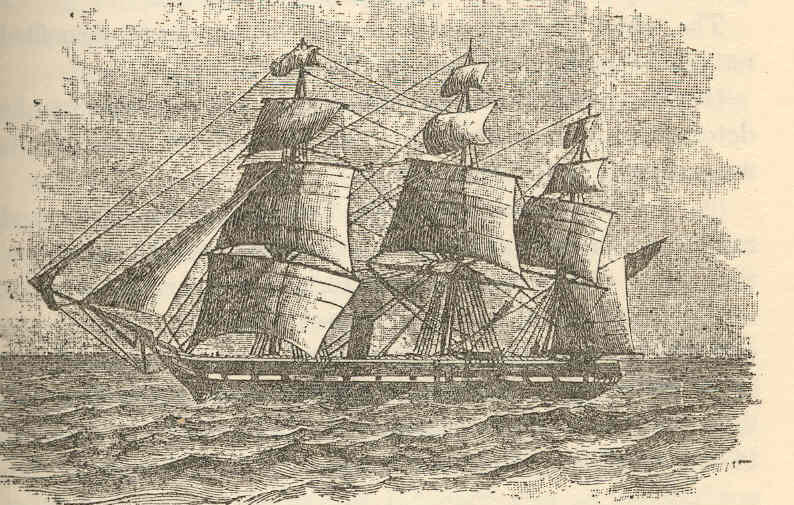
\includegraphics[width=0.55\linewidth]{images/book1/g8-challenger-sounding.jpg}

{\small HMS \emph{Challenger} bersiap mengukur kedalaman \omterm{def:g2:water-on-earth:ocean}{samudra}, 1872.
Gravir dari laporan-laporan ekspedisi itu, dimuat ulang dalam
W.~A.~Herdman, \emph{Founders of Oceanography} (1923); domain publik,
melalui Wikimedia Commons.}
% ledger: commons:challenger
\label{fig:g8:the-oceans:challenger}
\end{omfigure}

Sekarang kapal memetakan dasar \omterm{def:g2:water-on-earth:ocean}{laut} dengan bunyi. Sebuah alat di bawah
lambungnya memancarkan denyut bunyi yang singkat ke bawah; bunyi itu
memantul dari dasar dan kembali sebagai gema. Waktu yang diperlukan gema
itu menunjukkan kedalamannya, berulang-ulang, selagi kapal terus berlayar.
Inilah \emph{sonar}.
% ledger: nos:sonar

\begin{recall}
\omterm{def:g2:water-on-earth:salt-fresh}{Air asin} menutupi sebagian besar Bumi, dalam satu \omterm{def:g2:water-on-earth:ocean}{samudra} dunia yang
terbagi menjadi \omterm{def:g2:water-on-earth:ocean}{samudra-samudra} dan \omterm{def:g2:water-on-earth:ocean}{laut-laut} (\cref{ch:g2:water-on-earth}).
\omterm{def:g7:plate-tectonics:plate}{Lempeng-lempeng} saling menjauh di \omterm{def:g8:the-oceans:seafloor}{punggung samudra}, dan satu \omterm{def:g7:plate-tectonics:plate}{lempeng}
menunjam ke bawah \omterm{def:g7:plate-tectonics:plate}{lempeng} lain di palung (\cref{ch:g7:plate-tectonics}).
Di atas \omterm{def:g2:water-on-earth:ocean}{samudra}, angin bertiup dalam sabuk-sabuk yang besar: \omterm{def:g8:winds-global-circulation:global-winds}{angin pasat},
\omterm{def:g8:winds-global-circulation:global-winds}{angin baratan}, dan \omterm{def:g8:winds-global-circulation:global-winds}{angin timuran kutub}, yang dibelokkan oleh perputaran
Bumi (\cref{ch:g8:winds-global-circulation}).
\end{recall}

\section{Dasar samudra}

Seandainya air \omterm{def:g2:water-on-earth:ocean}{samudra} dapat dikuras habis, akan tampak seluruh \omterm{def:g1:landscapes-around-us:landscape}{bentang
alam} yang tersembunyi. Di sepanjang pantai, daratan berlanjut di bawah
\omterm{def:g2:water-on-earth:ocean}{laut} sebagai paparan yang landai dan dangkal. Lalu dasar \omterm{def:g2:water-on-earth:ocean}{laut} menukik
menuruni lereng yang curam sampai ke \omterm{def:g1:landscapes-around-us:landform}{dataran} yang luas dan datar,
berkilo-kilometer dalamnya. Rangkaian \omterm{def:g4:world-physical-map:range}{pegunungan} menjulang dari \omterm{def:g1:landscapes-around-us:landform}{dataran}
ini, dan di sana-sini palung yang sempit turun lebih dalam daripada
tempat mana pun di Bumi.
% ledger: edin:challenger-stations

\begin{omfigure}
\begin{tikzpicture}[font=\footnotesize, >={Stealth[length=2mm]}]
  \fill[omSea] (0,0) rectangle (15.6,-4.2);
  \fill[omLithAlluv] (0,0.6) -- (1.2,0.15) -- (1.6,0) -- (3.4,-0.35)
    .. controls (3.9,-0.55) and (4.1,-2.6) .. (4.7,-3.1)
    -- (6.6,-3.35) -- (7.6,-3.1) -- (8.3,-2.2) -- (8.6,-1.7) -- (8.75,-1.9) -- (8.9,-1.65) -- (9.2,-2.3) -- (10.0,-3.15)
    -- (11.6,-3.4) -- (12.6,-3.45) -- (13.05,-4.1) -- (13.35,-3.0) -- (14.2,-0.9) -- (14.8,0.7) -- (15.6,1.3)
    -- (15.6,-4.6) -- (0,-4.6) -- cycle;
  \draw[black!70] (0,0.6) -- (1.2,0.15) -- (1.6,0) -- (3.4,-0.35)
    .. controls (3.9,-0.55) and (4.1,-2.6) .. (4.7,-3.1)
    -- (6.6,-3.35) -- (7.6,-3.1) -- (8.3,-2.2) -- (8.6,-1.7) -- (8.75,-1.9) -- (8.9,-1.65) -- (9.2,-2.3) -- (10.0,-3.15)
    -- (11.6,-3.4) -- (12.6,-3.45) -- (13.05,-4.1) -- (13.35,-3.0) -- (14.2,-0.9) -- (14.8,0.7) -- (15.6,1.3);
  \draw[omRiver] (1.55,0) -- (14.45,0);
  \node[anchor=south] at (8,0.05) {permukaan laut};
  \node[align=center] at (2.6,-0.85) {paparan\\benua};
  \draw[->] (2.6,-0.55) -- (2.6,-0.25);
  \node[align=center, anchor=east] at (3.7,-2.0) {lereng\\benua};
  \draw[->] (3.75,-2.0) -- (4.1,-1.9);
  \node[align=center] at (5.7,-2.6) {dataran abisal};
  \node[align=center] at (8.75,-0.9) {punggung samudra};
  \draw[->] (8.75,-1.15) -- (8.75,-1.55);
  \node[align=center] at (11.1,-2.6) {dataran abisal};
  \node[align=center, anchor=west] at (13.5,-3.9) {palung\\samudra};
  \draw[->] (13.45,-3.9) -- (13.15,-3.9);
  \node[anchor=south] at (0.8,0.6) {benua};
  \node[anchor=south east] at (14.7,1.0) {pegunungan};
\end{tikzpicture}

{\small Bagian-bagian dasar \omterm{def:g2:water-on-earth:ocean}{samudra}, dari sebuah pantai ke \omterm{def:g2:water-on-earth:ocean}{samudra} lepas
dan ke pantai yang lain (sketsa: kedalaman dan lebarnya tidak berskala).}
\label{fig:g8:the-oceans:sketch}
\end{omfigure}

\begin{definition}[Bagian-bagian dasar samudra]\label{def:g8:the-oceans:seafloor}
\begin{itemize}
  \item Yang disebut \emph{paparan benua}\index{paparan benua} adalah tepi
        \omterm{def:g3:continents-and-oceans:continent}{benua} di bawah \omterm{def:g2:water-on-earth:ocean}{laut} yang dangkal dan landai.
  \item Yang disebut \emph{lereng benua}\index{lereng benua} adalah lereng
        curam yang menurun dari paparan ke dasar \omterm{def:g2:water-on-earth:ocean}{samudra} yang dalam.
  \item Yang disebut \emph{dataran abisal}\index{dataran abisal} adalah
        bagian dasar \omterm{def:g2:water-on-earth:ocean}{samudra} yang luas, sangat datar, dan dalam.
  \item Yang disebut \emph{punggung samudra}\index{punggung samudra} adalah
        rangkaian panjang \omterm{def:g4:world-physical-map:range}{pegunungan} bawah \omterm{def:g2:water-on-earth:ocean}{laut} yang menjulang dari \omterm{def:g1:landscapes-around-us:landform}{dataran}
        abisal.
  \item Yang disebut \emph{palung samudra}\index{palung samudra} adalah
        cekungan panjang, sempit, dan sangat dalam di dasar \omterm{def:g2:water-on-earth:ocean}{samudra},
        sering kali di dekat rangkaian \omterm{def:g4:world-physical-map:range}{pegunungan} atau pulau-pulau
        \omterm{def:g4:volcanoes-earthquakes-first-look:volcano}{gunung api}.
\end{itemize}
\end{definition}
% ledger: edin:challenger-stations, usgs:trench-depth

Rata-rata, kedalaman \omterm{def:g2:water-on-earth:ocean}{samudra} sekitar \qty{3700}{m}, hampir separuh tinggi
\omterm{def:g1:landscapes-around-us:landform}{gunung} tertinggi di daratan. Titik terdalamnya, Jurang Challenger di
Palung Mariana di \omterm{def:g2:water-on-earth:ocean}{Samudra} Pasifik, terletak hampir \qty{11000}{m} di
bawah permukaan.
% ledger: nos:ocean-depth, usgs:trench-depth, tht:everest


\begin{method}[Membaca profil dasar samudra]
\begin{enumerate}
  \item Bacalah sumbu-sumbunya: jarak secara mendatar, \omterm{def:g4:world-physical-map:altitude}{ketinggian} atau
        kedalaman secara tegak, dan perbesaran vertikalnya.
  \item Temukan \omterm{def:g4:world-physical-map:altitude}{permukaan laut} (\omterm{def:g4:world-physical-map:altitude}{ketinggian} 0) dan pantai-pantai tempat
        profil memotongnya.
  \item Ikuti dasar \omterm{def:g2:water-on-earth:ocean}{laut} dari sebuah pantai: paparan yang dangkal, lereng
        yang curam, lalu \omterm{def:g1:landscapes-around-us:landform}{dataran} yang dalam dan datar.
  \item Carilah apa yang menjulang dari \omterm{def:g1:landscapes-around-us:landform}{dataran} (punggung) atau turun di
        bawahnya (palung), lalu bacalah kedalamannya.
\end{enumerate}
\end{method}

\begin{example}[Melintasi Atlantik Selatan]
Pada profil atas, selewat pantai Amerika Selatan, dasar \omterm{def:g2:water-on-earth:ocean}{laut} turun sampai
lebih dari \qty{3000}{m} dalamnya dalam jarak kurang dari \qty{300}{km}.
\omterm{def:g8:the-oceans:seafloor}{Dataran abisal}, yang dalamnya antara \qty{3500}{m} dan \qty{5000}{m},
mengisi sebagian besar lebarnya. Di tengah perjalanan, sekitar
\qty{4400}{km} sepanjang profil, Punggung Tengah Atlantik menjulang sampai
sekitar \qty{2300}{m} di bawah permukaan: lebih dari \qty{2000}{m} di
atas \omterm{def:g1:landscapes-around-us:landform}{dataran}, rangkaian \omterm{def:g4:world-physical-map:range}{pegunungan} yang tersembunyi di bawah \omterm{def:g2:water-on-earth:ocean}{laut}. \omterm{def:g1:landscapes-around-us:landform}{Dataran}
itu kembali mendalam sampai lebih dari \qty{5000}{m} sebelum dasar \omterm{def:g2:water-on-earth:ocean}{laut}
naik ke Afrika.
\end{example}
% ledger: data:etopo1 (figdata/grade-8/seafloor_profile.py: ridge crest -2329 m at 4407 km; deepest -5295 m)

\begin{omfigure}
\begin{tikzpicture}
\begin{axis}[omsection, scale only axis, width=14cm, height=3.6cm, xmin=0, xmax=7569,
  ymin=-6000, ymax=1500, ytick={-6000,-4000,-2000,0}, xtick={0,1000,...,7000},
  xlabel={jarak sepanjang 30.5\textdegree\ LS, dari 59.5\textdegree\ BB (km)}, ylabel={ketinggian (m)},
  tick label style={font=\scriptsize}, label style={font=\small},
  yticklabel style={/pgf/number format/1000 sep={\,}}, xticklabel style={/pgf/number format/1000 sep={\,}},
  axis background/.style={fill=white}, clip=true]
  \fill[omSea] (axis cs:0,-6000) rectangle (axis cs:7569,0);
  \addplot[fill=omLithAlluv, draw=black!70, line width=0.5pt] table[x=km, y=elev_m] {figdata/out/grade-8-seafloor_profile-atlantic-rock.dat};
  \node[font=\scriptsize, align=center, fill=white, inner sep=1pt] at (axis cs:4407,-900) {Punggung Tengah Atlantik};
  \draw[-{Stealth[length=1.5mm]}] (axis cs:4407,-1250) -- (axis cs:4407,-2150);
  \node[font=\scriptsize] at (axis cs:2500,-5300) {dataran abisal};
  \node[font=\scriptsize] at (axis cs:6200,-5600) {dataran abisal};
  \node[font=\scriptsize, anchor=south west] at (axis cs:30,350) {Amerika Selatan};
  \node[font=\scriptsize, anchor=south east] at (axis cs:7380,350) {Afrika};
  \node[anchor=north] at (rel axis cs:0.75,0.97) {\omve{260}};
\end{axis}
\end{tikzpicture}

\medskip
\begin{tikzpicture}
\begin{axis}[omsection, scale only axis, width=7cm, height=3.6cm, xmin=0, xmax=3020,
  ymin=-6000, ymax=4500, ytick={-6000,-4000,-2000,0,2000,4000}, xtick={0,1000,2000,3000},
  xlabel={jarak sepanjang 20.5\textdegree\ LS (km)}, ylabel={ketinggian (m)},
  tick label style={font=\scriptsize}, label style={font=\small},
  yticklabel style={/pgf/number format/1000 sep={\,}}, xticklabel style={/pgf/number format/1000 sep={\,}},
  axis background/.style={fill=white}, clip=true]
  \fill[omSea] (axis cs:0,-6000) rectangle (axis cs:3020,0);
  \addplot[fill=omLithAlluv, draw=black!70, line width=0.5pt] table[x=km, y=elev_m] {figdata/out/grade-8-seafloor_profile-pacific-rock.dat};
  \node[font=\scriptsize, align=center, fill=white, inner sep=1pt] at (axis cs:1300,1600) {Palung Peru--Chili};
  \draw[-{Stealth[length=1.5mm]}] (axis cs:1750,1150) -- (axis cs:1870,-5000);
  \node[font=\scriptsize, anchor=west] at (axis cs:2600,3500) {Andes};
  \node[font=\scriptsize] at (axis cs:700,-5300) {dataran abisal};
  \node[anchor=north west] at (rel axis cs:0.01,0.98) {\omve{148}};
\end{axis}
\end{tikzpicture}

{\small Dua profil nyata dasar \omterm{def:g2:water-on-earth:ocean}{samudra}, dari relief ETOPO1 yang dibaca
setiap satu derajat \omterm{def:g6:latitude-longitude:longitude}{bujur}. Atas: melintasi Atlantik Selatan, dari Amerika
Selatan ke Afrika. Bawah: melintasi tepi Pasifik Amerika Selatan.
\omterm{def:g4:world-physical-map:altitude}{Ketinggiannya} diregangkan 260 dan 148 kali dibandingkan dengan jaraknya
(\emph{perbesaran vertikal}); tanpa itu, \omterm{def:g2:water-on-earth:ocean}{samudra} akan tampak setipis
selembar kertas. Dan karena hanya ada satu titik setiap derajat, palung
yang sempit itu tampak lebih dangkal daripada yang sebenarnya.}
% ledger: data:etopo1, earth:Rmean (figdata/grade-8/seafloor_profile.py)
\label{fig:g8:the-oceans:profiles}
\end{omfigure}


\section{Air yang asin}

Air \omterm{def:g2:water-on-earth:ocean}{laut} terasa asin karena ada garam-garam yang terlarut di dalamnya.
Sebagian besar garam itu berasal dari \omterm{def:g3:stones-pebbles-sand:rock}{batuan} \omterm{def:g3:continents-and-oceans:continent}{benua}: \omterm{def:g4:clouds-rain-snow:precipitation}{hujan} perlahan-lahan
mengikis \omterm{def:g3:stones-pebbles-sand:rock}{batuan}, dan \omterm{def:g1:landscapes-around-us:water}{sungai} membawa garam-garamnya yang terlarut ke \omterm{def:g2:water-on-earth:ocean}{laut}.
Sebagian lagi berasal dari mata air panas di dasar \omterm{def:g2:water-on-earth:ocean}{samudra}.
% ledger: nos:salinity-varies

\begin{definition}[Salinitas]\label{def:g8:the-oceans:salinity}
Yang disebut \emph{salinitas}\index{salinitas} air \omterm{def:g2:water-on-earth:ocean}{laut} adalah massa
garam yang terlarut dalam satu kilogram air \omterm{def:g2:water-on-earth:ocean}{laut}. Rata-rata besarnya
sekitar \qty{35}{g} per kilogram: \qty{3.5}{\%} dari massa air \omterm{def:g2:water-on-earth:ocean}{laut}
adalah garam.
\end{definition}
% ledger: nos:salinity-varies

\omterm{def:g8:the-oceans:salinity}{Salinitas} tidak sama di mana-mana. Ketika air \omterm{def:g2:water-on-earth:ocean}{laut} menguap, airnya pergi
tetapi garamnya tertinggal: di tempat Matahari terik dan \omterm{def:g4:clouds-rain-snow:precipitation}{hujan} jarang,
\omterm{def:g2:water-on-earth:ocean}{laut} menjadi lebih asin. Di tempat banyak \omterm{def:g4:clouds-rain-snow:precipitation}{hujan} turun, atau tempat \omterm{def:g1:landscapes-around-us:water}{sungai}
besar bermuara, \omterm{def:g2:water-on-earth:ocean}{laut} kurang asin. Ketika air \omterm{def:g2:water-on-earth:ocean}{laut} membeku menjadi es \omterm{def:g2:water-on-earth:ocean}{laut},
garamnya tertinggal di air di sekitarnya, yang juga menjadi lebih asin.
Secara keseluruhan, \omterm{def:g8:the-oceans:salinity}{salinitas} rendah di dekat \omterm{def:g3:continents-and-oceans:equator}{khatulistiwa}, tempat banyak
\omterm{def:g4:clouds-rain-snow:precipitation}{hujan} turun, dan di dekat \omterm{def:g3:continents-and-oceans:poles}{kutub}; \omterm{def:g8:the-oceans:salinity}{salinitas} paling tinggi di \omterm{def:g6:latitude-longitude:latitude}{lintang}
tengah, di bawah sabuk-sabuk kering di dekat \ang{30}.
% ledger: nos:salinity-varies, nos:sea-ice-salt, mo:three-cells

\begin{omfigure}
\begin{tikzpicture}[font=\footnotesize, >={Stealth[length=2mm]}]
  \fill[omSea] (0,0) rectangle (13,-1.6);
  \draw[omRiver, line width=0.8pt] (0,0) -- (13,0);
  % left: dry belt, evaporation
  \fill[yellow!80!orange] (1.2,3.0) circle (0.35);
  \foreach \x in {1.0,1.8,2.6,3.4} \draw[->, black!50, line width=0.9pt, decorate, decoration={snake, amplitude=0.6mm, segment length=3mm}] (\x,0.15) -- (\x,1.6);
  \node[align=center] at (2.3,2.2) {penguapan kuat,\\sedikit hujan};
  \node[align=center, fill=white, inner sep=1.5pt] at (2.3,-0.8) {\textbf{lebih asin}};
  % middle: rain
  \fill[black!20] (5.2,2.9) ellipse [x radius=1.3, y radius=0.4];
  \foreach \x in {4.4,4.8,...,6.0} \draw[omRiver] (\x,2.45) -- (\x-0.2,0.25);
  \node[align=center, fill=white, inner sep=1.5pt] at (5.2,-0.8) {\textbf{kurang asin}};
  \node at (5.2,3.55) {hujan lebat};
  % right: river mouth and sea ice
  \fill[omLithAlluv] (7.4,0) -- (9.6,0) -- (9.6,0.6) -- (7.4,0.35) -- cycle;
  \draw[omRiver, line width=2pt, ->] (9.4,0.45) -- (7.9,0.2);
  \node[anchor=south] at (8.6,0.65) {sungai};
  \node[align=center, fill=white, inner sep=1.5pt] at (8.6,-0.8) {\textbf{kurang asin}};
  \fill[white, draw=omCold] (10.6,0.25) -- (12.6,0.25) -- (12.4,-0.25) -- (10.8,-0.25) -- cycle;
  \node[anchor=south] at (11.6,0.3) {es laut terbentuk};
  \node[align=center, fill=white, inner sep=1.5pt] at (11.6,-0.95) {\textbf{lebih asin}\\(garam tertinggal)};
\end{tikzpicture}

{\small Apa yang mengubah \omterm{def:g8:the-oceans:salinity}{salinitas} \omterm{def:g2:water-on-earth:ocean}{laut}: penguapan dan pembekuan
meninggalkan garamnya; \omterm{def:g4:clouds-rain-snow:precipitation}{hujan} dan \omterm{def:g1:landscapes-around-us:water}{sungai} menambahkan \omterm{def:g2:water-on-earth:salt-fresh}{air tawar}.}
% ledger: nos:salinity-varies, nos:sea-ice-salt
\label{fig:g8:the-oceans:salinity}
\end{omfigure}

\begin{omfigure}
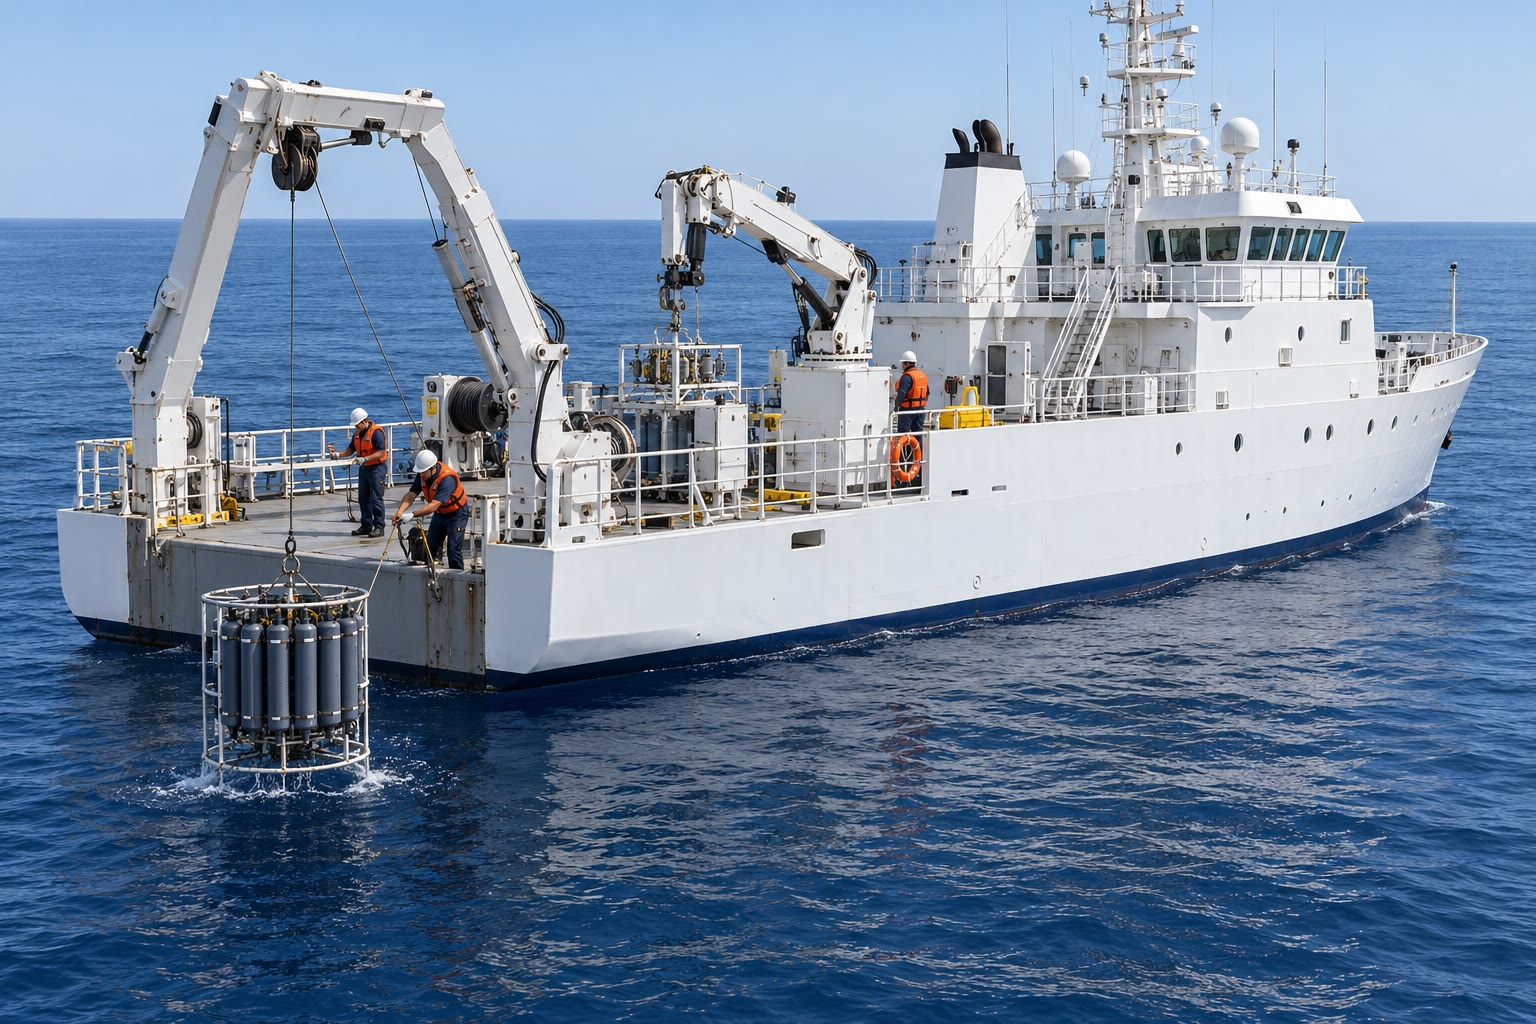
\includegraphics[width=0.58\linewidth]{images/book1/ai/g8-research-ship.jpg}

{\small Sebuah kapal penelitian menurunkan kerangka berisi botol-botol
pengambil contoh ke dalam \omterm{def:g2:water-on-earth:ocean}{laut}, untuk membawa naik air dari kedalaman dan
mengukur keasinan serta suhunya (ilustrasi AI dari suatu adegan umum).}
\label{fig:g8:the-oceans:ship}
\end{omfigure}

\section{Arus di permukaan}

\omterm{def:g2:water-on-earth:ocean}{Samudra} tidak pernah diam. Angin menyeret permukaannya dan membuat airnya
bergerak: \omterm{def:g8:winds-global-circulation:global-winds}{angin pasat} yang tetap mendorongnya ke barat di dekat
\omterm{def:g3:continents-and-oceans:equator}{khatulistiwa}, dan \omterm{def:g8:winds-global-circulation:global-winds}{angin baratan} mendorongnya ke timur di \omterm{def:g6:latitude-longitude:latitude}{lintang} tengah.
Seperti angin, air yang bergerak itu dibelokkan oleh perputaran Bumi: ke
kanan di \omterm{def:g3:continents-and-oceans:equator}{belahan bumi utara}, ke kiri di \omterm{def:g3:continents-and-oceans:equator}{belahan bumi selatan}.
% ledger: nos:gyres

\begin{definition}[Arus laut dan pilin samudra]\label{def:g8:the-oceans:current}
Yang disebut \emph{arus laut}\index{arus laut} adalah gerakan air \omterm{def:g2:water-on-earth:ocean}{laut}
yang tetap ke satu arah, seperti \omterm{def:g1:landscapes-around-us:water}{sungai} di dalam \omterm{def:g2:water-on-earth:ocean}{samudra}. Yang disebut
\emph{pilin samudra}\index{pilin samudra} adalah lingkaran arus \omterm{def:g2:water-on-earth:ocean}{laut} yang
sangat besar yang berputar mengelilingi sebuah cekungan \omterm{def:g2:water-on-earth:ocean}{samudra}.
\end{definition}
% ledger: nos:gyre-def, nos:gyres
\phantomsection\label{def:g8:the-oceans:gyre}

Ada lima \omterm{def:g8:the-oceans:current}{pilin samudra} yang besar: di Atlantik Utara dan Atlantik Selatan,
di Pasifik Utara dan Pasifik Selatan, serta di \omterm{def:g2:water-on-earth:ocean}{Samudra} Hindia. \omterm{def:g8:the-oceans:current}{Pilin} di
\omterm{def:g3:continents-and-oceans:equator}{belahan bumi utara} berputar searah jarum jam, sedangkan \omterm{def:g8:the-oceans:current}{pilin} di \omterm{def:g3:continents-and-oceans:equator}{belahan
bumi selatan} berlawanan arah jarum jam. Di sisi barat setiap \omterm{def:g2:water-on-earth:ocean}{samudra}, arus
\omterm{def:g8:the-oceans:current}{pilinnya} sempit dan cepat; di sisi timur, arusnya lebar dan lambat.
% ledger: nos:gyres

\begin{inthelab}[Pilin di dalam piring]
Di dalam rumah, isilah sebuah piring bundar yang besar dengan air dan
taburkan sejumput merica di permukaannya. Tiuplah perlahan dan terus
melintasi piring itu lewat sedotan, selalu ke arah yang sama, di dekat
salah satu tepinya. Perhatikan mericanya: air di dekat permukaan mulai
bergerak mengikuti tiupanmu, dan tak lama kemudian seluruh permukaan
berputar melingkar mengelilingi piring.
\end{inthelab}

\begin{omfigure}
\begin{tikzpicture}
\begin{axis}[ommap, width=\linewidth, xmin=-180, xmax=180, ymin=-65, ymax=70,
  xtick={-180,-120,...,180}, ytick={-60,-30,0,30,60},
  xticklabels={$180^\circ$,$120^\circ$BB,$60^\circ$BB,$0^\circ$,$60^\circ$BT,$120^\circ$BT,$180^\circ$},
  yticklabels={$60^\circ$LS,$30^\circ$LS,$0^\circ$,$30^\circ$LU,$60^\circ$LU},
  tick label style={font=\scriptsize}]
  \addplot[fill=omLithAlluv, draw=black!45, line width=0.2pt] table {figdata/out/shared-geo-land.dat};
  \addplot[omWarm, line width=1.3pt] table {figdata/out/grade-8-ocean_currents-gyres-warm.dat};
  \addplot[omCold, line width=1.3pt] table {figdata/out/grade-8-ocean_currents-gyres-cold.dat};
  \addplot[quiver={u=\thisrow{u}, v=\thisrow{v}}, -{Stealth[length=2.6mm, width=2.2mm]}, omWarm, line width=1.3pt]
    table[x=lon, y=lat] {figdata/out/grade-8-ocean_currents-heads-warm.dat};
  \addplot[quiver={u=\thisrow{u}, v=\thisrow{v}}, -{Stealth[length=2.6mm, width=2.2mm]}, omCold, line width=1.3pt]
    table[x=lon, y=lat] {figdata/out/grade-8-ocean_currents-heads-cold.dat};
  \node[font=\scriptsize\bfseries, fill=white, inner sep=1pt, anchor=east] at (axis cs:-72,40) {Arus Teluk};
  \node[font=\scriptsize\bfseries, fill=white, inner sep=1pt, anchor=west] at (axis cs:-12,25) {Arus Kanari};
\end{axis}
\end{tikzpicture}

{\small Lima \omterm{def:g8:the-oceans:current}{pilin samudra} yang besar, disederhanakan: searah jarum jam di
\omterm{def:g3:continents-and-oceans:equator}{belahan bumi utara}, berlawanan arah jarum jam di \omterm{def:g3:continents-and-oceans:equator}{belahan bumi selatan}.
Merah: arus hangat, yang datang dari \omterm{def:g5:weather-and-climate:tropics}{daerah tropis}; biru: arus dingin, yang
datang dari \omterm{def:g6:latitude-longitude:latitude}{lintang} yang lebih tinggi. \omterm{def:g8:the-oceans:current}{Pilin} Atlantik Utara dibatasi oleh
Arus Teluk di sebelah barat dan Arus Kanari di sebelah timur.}
% ledger: nos:gyres, data:ne-land (figdata/grade-8/ocean_currents.py)
\label{fig:g8:the-oceans:gyres}
\end{omfigure}

Arus yang paling terkenal di antara semuanya adalah Arus Teluk. Arus ini
meninggalkan Teluk Meksiko, mengalir ke utara di sepanjang pantai Florida,
berbelok ke timur di lepas pantai North Carolina, dan menyeberangi
Atlantik ke arah timur laut. Airnya yang hangat bergerak rata-rata dengan
kecepatan sekitar \qty{6.4}{km} per jam, sampai sekitar \qty{9}{km} per jam
di permukaan, dan membawa lebih banyak air daripada semua \omterm{def:g1:landscapes-around-us:water}{sungai} di dunia
digabungkan. Arus ini membuat pantai timur Florida lebih hangat pada musim
dingin dan membawa udara yang sejuk ke Eropa barat.
% ledger: nos:gulf-stream, nos:gyres

\begin{omfigure}
\begin{minipage}[c]{0.5\linewidth}\centering
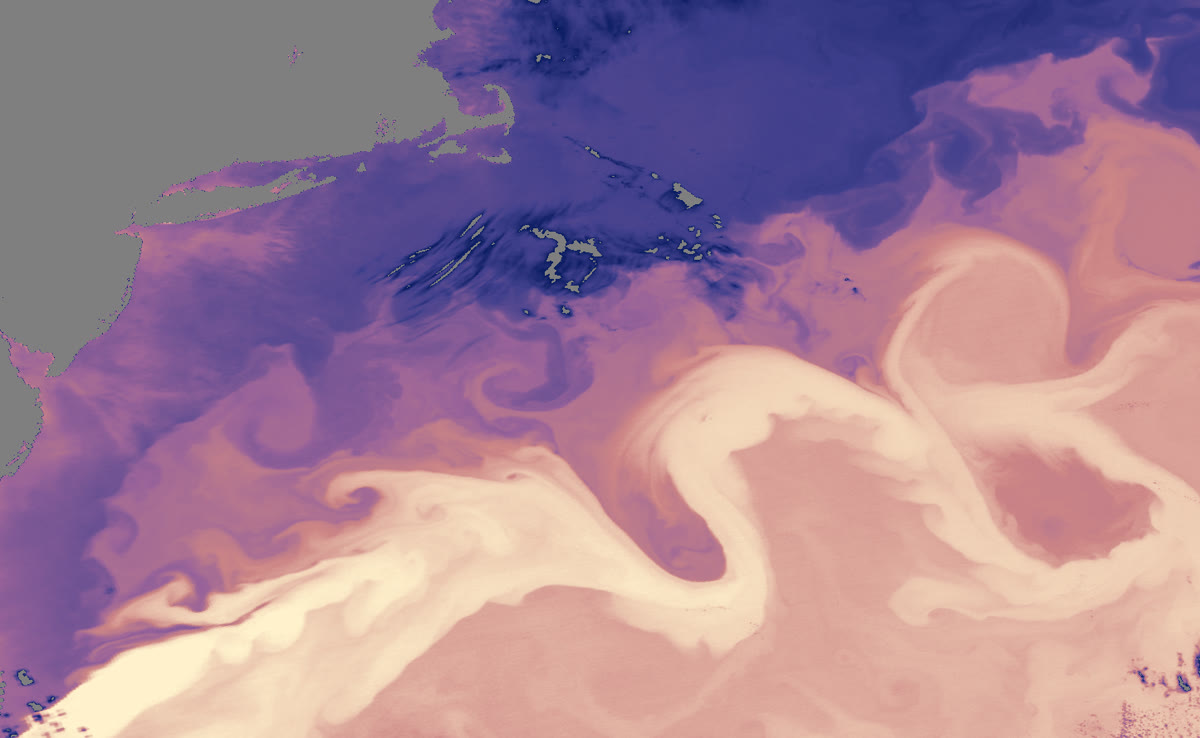
\includegraphics[width=\linewidth]{images/book1/g8-gulf-stream-sst.jpg}
\end{minipage}\hfill
\begin{minipage}[c]{0.46\linewidth}\raggedright
{\small Suhu \omterm{def:g4:world-physical-map:altitude}{permukaan laut} di lepas pantai timur Amerika Utara, yang
diukur oleh satelit Aqua milik NASA pada 18~April 2005. Arus Teluk adalah
pita air hangat (warna terang, sampai sekitar \qty{23}{\degreeCelsius})
yang berkelok dari kiri bawah ke arah kanan, di antara air yang lebih
dingin (gelap, sampai sekitar \qty{-1}{\degreeCelsius}); daratan berwarna
kelabu. NASA (domain publik, melalui Wikimedia Commons).}
\end{minipage}
% ledger: commons:gulf-sst
\label{fig:g8:the-oceans:gulf}
\end{omfigure}


\section{Arus dalam dan panas samudra}

Angin menggerakkan arus di permukaan. Jauh di bawah, dalam kegelapan yang
dingin di \omterm{def:g2:water-on-earth:ocean}{samudra} dalam, air juga bergerak, jauh lebih lambat. Di
Atlantik Utara bagian paling utara, air hangat yang dibawa Arus Teluk
melepaskan panasnya ke udara yang dingin; setelah mendingin, dan menjadi
lebih asin ketika es \omterm{def:g2:water-on-earth:ocean}{laut} terbentuk, air itu menjadi lebih rapat dan
tenggelam ke dasar. Air yang dingin dan asin ini merayap ke selatan di
sepanjang dasar \omterm{def:g2:water-on-earth:ocean}{samudra}, sampai ke Antarktika, lalu masuk ke \omterm{def:g2:water-on-earth:ocean}{Samudra} Hindia
dan \omterm{def:g2:water-on-earth:ocean}{Samudra} Pasifik, tempat air itu perlahan-lahan naik dan kembali di
permukaan. Setetes air dapat memerlukan sekitar \num{1000} tahun untuk
menempuh satu kali putaran lingkaran besar ini, yaitu \emph{sabuk konveyor
\omterm{def:g2:water-on-earth:ocean}{samudra} global}.
% ledger: nos:conveyor, nos:sea-ice-salt

\begin{omfigure}
\begin{tikzpicture}
\begin{axis}[ommap, width=\linewidth, xmin=-180, xmax=180, ymin=-65, ymax=70,
  xtick={-180,-120,...,180}, ytick={-60,-30,0,30,60},
  xticklabels={$180^\circ$,$120^\circ$BB,$60^\circ$BB,$0^\circ$,$60^\circ$BT,$120^\circ$BT,$180^\circ$},
  yticklabels={$60^\circ$LS,$30^\circ$LS,$0^\circ$,$30^\circ$LU,$60^\circ$LU},
  tick label style={font=\scriptsize}]
  \addplot[fill=omLithAlluv, draw=black!45, line width=0.2pt] table {figdata/out/shared-geo-land.dat};
  \addplot[omWarm, line width=1.3pt] table {figdata/out/grade-8-conveyor-surface.dat};
  \addplot[omCold, line width=1.3pt, dashed] table {figdata/out/grade-8-conveyor-deep.dat};
  \addplot[quiver={u=\thisrow{u}, v=\thisrow{v}}, -{Stealth[length=2.6mm, width=2.2mm]}, omWarm, line width=1.3pt]
    table[x=lon, y=lat] {figdata/out/grade-8-conveyor-heads-surface.dat};
  \addplot[quiver={u=\thisrow{u}, v=\thisrow{v}}, -{Stealth[length=2.6mm, width=2.2mm]}, omCold, line width=1.3pt]
    table[x=lon, y=lat] {figdata/out/grade-8-conveyor-heads-deep.dat};
  \node[font=\scriptsize\bfseries, fill=white, inner sep=1pt, anchor=west] at (axis cs:4,64) {tenggelam};
  \node[font=\scriptsize\bfseries, fill=white, inner sep=1pt, anchor=south] at (axis cs:163,11) {naik};
\end{axis}
\end{tikzpicture}

{\small Sabuk konveyor \omterm{def:g2:water-on-earth:ocean}{samudra} global, disederhanakan menjadi satu
lingkaran saja (sketsa). Merah: air hangat di permukaan; biru, putus-putus:
air yang dingin dan asin yang merayap di sepanjang dasar \omterm{def:g2:water-on-earth:ocean}{samudra} yang
dalam. Air tenggelam di Atlantik Utara bagian paling utara, di antara
Greenland dan Norwegia, lalu naik di Pasifik (dan, tidak digambar, di
\omterm{def:g2:water-on-earth:ocean}{Samudra} Hindia).}
% ledger: nos:conveyor, data:ne-land (figdata/grade-8/conveyor.py)
\end{omfigure}

\begin{example}[Seberapa lambat air dalam?]\label{ex:g8:the-oceans:deep-speed}
Lingkaran yang digambar pada \omterm{def:g2:drawing-to-map:map}{peta} panjangnya kira-kira \qty{70000}{km}.
Jika setetes air memerlukan sekitar \num{1000} tahun untuk mengelilinginya,
air itu bergerak rata-rata sekitar
$\num{70000} \div \num{1000} = \qty{70}{km}$ setahun, yaitu sekitar
\qty{200}{m} sehari. Arus Teluk, dengan kecepatan \qty{6.4}{km} per jam,
menempuh sekitar \qty{150}{km} dalam sehari: dalam sekitar 11 jam, arus
itu menempuh jarak sejauh yang ditempuh air dalam selama setahun penuh.
% ledger: nos:conveyor, nos:gulf-stream, earth:Rmean (loop length and speeds computed in figdata/grade-8/conveyor.py)
\end{example}

Bersama-sama, arus permukaan dan arus dalam membawa panas: air hangat
mengalir dari \omterm{def:g5:weather-and-climate:tropics}{daerah tropis} ke arah \omterm{def:g3:continents-and-oceans:poles}{kutub}, dan air dingin mengalir kembali
ke arah \omterm{def:g3:continents-and-oceans:equator}{khatulistiwa}. Seperti angin, \omterm{def:g2:water-on-earth:ocean}{samudra} meratakan pemanasan Bumi oleh
Matahari yang tidak merata.
% ledger: nos:conveyor, nos:gulf-stream, mo:global-circ

\section{Latihan}

\begin{exercise}[$\star$]\label{exo:g8:the-oceans:1}
Urutkan bagian-bagian dasar \omterm{def:g2:water-on-earth:ocean}{samudra} ini sesuai urutan yang dijumpai
sebuah kapal selam ketika meninggalkan pantai menuju tengah Atlantik:
\omterm{def:g8:the-oceans:seafloor}{dataran abisal}; \omterm{def:g8:the-oceans:seafloor}{lereng benua}; \omterm{def:g8:the-oceans:seafloor}{punggung samudra}; \omterm{def:g8:the-oceans:seafloor}{paparan benua}.
\end{exercise}

\begin{exercise}[$\star$]\label{exo:g8:the-oceans:2}
Benar atau salah? Perbaiki kalimat yang salah. (a) Rata-rata, kedalaman
\omterm{def:g2:water-on-earth:ocean}{samudra} sekitar \qty{37}{km}. (b) \omterm{def:g8:the-oceans:current}{Pilin samudra} di \omterm{def:g3:continents-and-oceans:equator}{belahan bumi utara}
berputar searah jarum jam. (c) Penguapan membuat air \omterm{def:g2:water-on-earth:ocean}{laut} kurang asin.
(d) Arus Teluk adalah arus hangat.
\end{exercise}

\begin{exercise}[$\star$]\label{exo:g8:the-oceans:3}
Berikan istilah untuk setiap uraian: (a) rangkaian panjang \omterm{def:g4:world-physical-map:range}{pegunungan} di
bawah \omterm{def:g2:water-on-earth:ocean}{laut}; (b) massa garam dalam satu kilogram air \omterm{def:g2:water-on-earth:ocean}{laut}; (c) lingkaran
\omterm{def:g8:the-oceans:current}{arus laut} yang sangat besar; (d) cekungan panjang, sempit, dan sangat
dalam di dasar \omterm{def:g2:water-on-earth:ocean}{samudra}.
\end{exercise}

\begin{exercise}[$\star$]\label{exo:g8:the-oceans:4}
Pada \omterm{def:g2:drawing-to-map:map}{peta} \omterm{def:g8:the-oceans:current}{pilin samudra}: (a) ke arah mana \omterm{def:g8:the-oceans:current}{pilin} Atlantik Selatan
berputar? (b) Sebutkan satu arus hangat dan satu arus dingin di Atlantik
Utara. (c) Angin apa yang mendorong air ke barat di dekat \omterm{def:g3:continents-and-oceans:equator}{khatulistiwa}?
\end{exercise}

\begin{exercise}[$\star\star$]\label{exo:g8:the-oceans:5}
Sebuah contoh air \omterm{def:g2:water-on-earth:ocean}{laut} seberat \qty{1}{kg} mengandung \qty{35}{g} garam.
(a) Berapa persen massanya yang berupa garam? (b) Berapa gram garam yang
ada dalam \qty{20}{kg} air ini? (c) Berapa kilogram air \omterm{def:g2:water-on-earth:ocean}{laut} yang
mengandung \qty{1}{kg} garam?
\end{exercise}

\begin{exercise}[$\star\star$]\label{exo:g8:the-oceans:6}
Sonar sebuah kapal memancarkan denyut bunyi tegak lurus ke bawah. Gemanya
kembali \qty{6}{s} kemudian. Di dalam air \omterm{def:g2:water-on-earth:ocean}{laut}, bunyi merambat sekitar
\qty{1500}{m} setiap detik. (a) Berapa jauh bunyi merambat dalam
\qty{6}{s}? (b) Mengapa kedalamannya hanya separuh jarak ini? (c) Berapa
kedalamannya? (d) Di atas bagian dasar \omterm{def:g2:water-on-earth:ocean}{samudra} yang mana kapal itu mungkin
berada?
\end{exercise}

\begin{exercise}[$\star\star$]\label{exo:g8:the-oceans:7}
Gunakan profil yang melintasi Atlantik Selatan. (a) Kira-kira berapa
kedalaman \omterm{def:g8:the-oceans:seafloor}{dataran abisalnya}? (b) Pada jarak berapa sepanjang profil
letak puncak Punggung Tengah Atlantik, dan berapa kedalamannya? (c) Berapa
meter punggung itu menjulang di atas \omterm{def:g1:landscapes-around-us:landform}{dataran}? (d) Mengapa profil itu
memerlukan perbesaran vertikal?
\end{exercise}

\begin{exercise}[$\star\star$]\label{exo:g8:the-oceans:8}
\omterm{def:g2:water-on-earth:ocean}{Laut} A terletak di antara dua \omterm{def:g5:weather-and-climate:desert}{gurun}: hampir tidak pernah \omterm{def:g4:clouds-rain-snow:precipitation}{hujan} di sana
dan tidak ada \omterm{def:g1:landscapes-around-us:water}{sungai} besar yang bermuara ke dalamnya. \omterm{def:g2:water-on-earth:ocean}{Laut} B, di wilayah
yang banyak \omterm{def:g4:clouds-rain-snow:precipitation}{hujan}, menerima banyak \omterm{def:g1:landscapes-around-us:water}{sungai} besar. Jelaskan mana di antara
keduanya yang lebih asin daripada \omterm{def:g2:water-on-earth:ocean}{samudra} lepas, dan mana yang kurang
asin. Gunakan kata-kata \emph{penguapan}, \emph{\omterm{def:g2:water-on-earth:salt-fresh}{air tawar}}, \emph{garam
tertinggal}.
\end{exercise}

\begin{exercise}[$\star\star$]\label{exo:g8:the-oceans:9}
Sebuah pesan di dalam botol dilemparkan ke \omterm{def:g2:water-on-earth:ocean}{laut} di lepas pantai Florida.
(a) Arus mana yang pertama kali membawanya, dan ke arah mana? (b) Ke arah
mana botol itu kemudian menyeberangi Atlantik? (c) Jika botol itu terus
mengelilingi \omterm{def:g8:the-oceans:current}{pilin}, di sepanjang pantai mana botol itu akan bergerak ke
selatan? (d) Apakah arus ini hangat atau dingin?
\end{exercise}

\begin{exercise}[$\star\star$]\label{exo:g8:the-oceans:10}
Arus Teluk bergerak rata-rata dengan kecepatan sekitar \qty{6.4}{km} per
jam. (a) Berapa jauh airnya bergerak dalam satu hari? (b) Dalam satu
minggu? (c) Bandingkan dengan orang yang berjalan kaki dengan kecepatan
\qty{5}{km} per jam.
\end{exercise}

\begin{exercise}[$\star\star\star$]\label{exo:g8:the-oceans:11}
Rata-rata, kedalaman \omterm{def:g2:water-on-earth:ocean}{samudra} sekitar \qty{3700}{m}, dan titik terdalamnya
hampir \qty{11000}{m}. (a) Tuliskan kedua kedalaman itu dalam kilometer.
(b) Berapa kali lebih dalam titik terdalam itu dibandingkan dengan
rata-ratanya? Bulatkan sampai satu tempat desimal. (c) Gema sonar dari
titik terdalam: berapa detik yang diperlukannya untuk kembali, dengan
\qty{1500}{m} setiap detik? (d) Setetes air sabuk konveyor tenggelam di
Atlantik Utara. Jika air itu memerlukan sekitar \num{1000} tahun untuk
menempuh satu putaran, berapa tahun itu dalam pangkat sepuluh?
\end{exercise}

\begin{exercise}[$\star\star\star$]\label{exo:g8:the-oceans:12}
Sabuk konveyor besar \omterm{def:g2:water-on-earth:ocean}{samudra} dalam bermula di \omterm{def:g2:water-on-earth:ocean}{Laut} Norwegia, di lepas
pantai Norwegia, tempat air hangat yang dibawa Arus Teluk melepaskan
panasnya ke udara yang dingin. (a) Dengan memakai \omterm{def:g2:drawing-to-map:map}{peta} \omterm{def:g8:the-oceans:current}{pilin samudra} dan
isi bab ini, jelaskan langkah demi langkah bagaimana air hangat itu
datang ke sana dari \omterm{def:g5:weather-and-climate:tropics}{daerah tropis}, dan angin apa yang mendorongnya.
(b) Jelaskan mengapa air itu kemudian tenggelam. (c) Ke mana air itu
pergi sesudahnya?
\end{exercise}

\section{Soal: Pelampung hanyut}

\begin{problem}[{Soal akhir pekan --- sebuah pelampung hanyut dilepaskan
di lepas pantai Florida dan terbawa mengelilingi pilin Atlantik Utara;
perjalanannya diikuti tahap demi tahap, dan waktu yang diperlukannya untuk
satu kali putaran dihitung}]
\label{pb:g8:the-oceans:1}
% ledger: nos:drifter, nos:gulf-stream, nos:gyres (figdata/grade-8/ocean_currents.py; the leg lengths are rounded, the speeds of legs B to D are exercise data)
Para ilmuwan melepaskan sebuah pelampung hanyut di lepas pantai Florida.
Pelampung itu mengapung tepat di bawah permukaan, bergerak mengikuti arus,
dan mengirimkan posisinya ke satelit. Baterainya bertahan sekitar satu
tahun. \omterm{def:g2:drawing-to-map:map}{Peta} menunjukkan keempat tahap perjalanannya mengelilingi \omterm{def:g8:the-oceans:current}{pilin}
Atlantik Utara.

\begin{center}
\begin{tikzpicture}
\begin{axis}[ommap, width=11.5cm, xmin=-95, xmax=0, ymin=5, ymax=55,
  xtick={-90,-60,-30,0}, ytick={10,30,50},
  xticklabels={$90^\circ$BB,$60^\circ$BB,$30^\circ$BB,$0^\circ$},
  yticklabels={$10^\circ$LU,$30^\circ$LU,$50^\circ$LU},
  tick label style={font=\scriptsize}]
  \addplot[fill=omLithAlluv, draw=black!45, line width=0.2pt] table {figdata/out/shared-geo-land.dat};
  \addplot[black, line width=1pt, densely dashed, postaction={decorate, decoration={markings,
      mark=between positions 0.04 and 0.98 step 0.08 with {\arrow{Stealth[length=2mm]}}}}]
    table[x=lon, y=lat] {figdata/out/grade-8-ocean_currents-buoy.dat};
  \addplot[only marks, mark=*, mark size=2.2pt, omDef] coordinates {(-79.5,26)};
  \node[font=\scriptsize\bfseries, anchor=east, fill=white, inner sep=1pt] at (axis cs:-81,26) {pelepasan};
  \addplot[only marks, mark=none, nodes near coords, point meta=explicit symbolic,
    every node near coord/.style={anchor=center, font=\footnotesize\bfseries, circle, fill=white, draw, inner sep=1pt}]
    table[x=lon, y=lat, meta=name] {figdata/out/grade-8-ocean_currents-buoy-legs.dat};
\end{axis}
\end{tikzpicture}

\medskip
{\small
\begin{tabular}{|c|l|c|c|}
\hline
tahap & arus & panjang (km) & kecepatan rata-rata (km per hari) \\
\hline
A & Arus Teluk & 3800 & 100 \\
B & Arus Atlantik Utara & 2100 & 20 \\
C & Arus Kanari & 3100 & 20 \\
D & Arus \omterm{def:g3:continents-and-oceans:equator}{Khatulistiwa} Utara & 6100 & 20 \\
\hline
\end{tabular}}
\end{center}

\noindent\textbf{Bagian I --- Pelepasan.}\par\nopagebreak
\begin{enumerate}[beginpenalty=10000]
  \item Di \omterm{def:g2:water-on-earth:ocean}{samudra} mana, dan di \omterm{def:g3:continents-and-oceans:equator}{belahan bumi} mana, pelampung itu dilepaskan?
  \item Ke arah mana \omterm{def:g8:the-oceans:current}{pilin} itu berputar? Apakah pelampung itu mula-mula
        terbawa ke utara atau ke selatan?
  \item Apakah air pada tahap A hangat atau dingin? Dan pada tahap C?
        Jelaskan.
  \item Angin apa yang menggerakkan arus pada tahap B? Pada tahap D?
\end{enumerate}

\noindent\textbf{Bagian II --- Mengelilingi pilin.}\par\nopagebreak
\begin{enumerate}[resume, beginpenalty=10000]
  \item Berapa hari yang diperlukan untuk tahap A?
  \item Berapa hari yang diperlukan untuk tahap B, C, dan D?
  \item Berapa panjang total perjalanan mengelilingi \omterm{def:g8:the-oceans:current}{pilin} itu?
  \item Mengapa tahap A jauh lebih cepat daripada tahap-tahap lainnya?
\end{enumerate}

\noindent\textbf{Bagian III --- Lamanya perjalanan.}\par\nopagebreak
\begin{enumerate}[resume, beginpenalty=10000]
  \item Berapa hari yang diperlukan pelampung itu untuk satu kali
        mengelilingi \omterm{def:g8:the-oceans:current}{pilin}?
  \item Jika satu bulan dianggap 30 hari, berapa bulan itu? Bulatkan
        sampai bulan bulat terdekat.
  \item Pada tahap mana baterainya akan habis, setelah sekitar satu tahun
        (365 hari)?
  \item Berapa bulan lagi daya baterai yang diperlukan pelampung itu agar
        dapat mengirimkan posisinya sepanjang seluruh putaran?
\end{enumerate}
\end{problem}
